\documentclass{article}
\usepackage[utf8]{inputenc}
\usepackage{graphicx}
\usepackage{hyperref}
\usepackage{listings}
\usepackage{float}
\usepackage[T2A,T1]{fontenc}
\usepackage[russian,french]{babel}
\usepackage{tikz}
\begin{document}
\title{Données Séquentielles et Symboliques: Translittération automatique}

\author{Alexandre Bérard, Mathias Millet, Charles Robin}
\maketitle
\begin{abstract}
\end{abstract}
\vspace{0.5em}
\section{Introduction}

La translittération est le fait de traduire, entre deux langues dont les graphèmes diffèrent\footnote{Un graphème est l'unité de l'écrit correspondant au phonème, une unité de prononciation orale}, un mot ayant la même (ou presque) prononciation dans les deux langues. C'est surtout le cas pour le vocabulaire technique, qui conserve  la même prononciation entre plusieurs langues, mais dont la transcription va varier (en particulier lorsque les langues sont écrites avec des alphabets différents).

La translitération trouve un interêt lorsqu'elle est effectuée de manière automatique. En effet, avec l'aparition de nouveaux termes techniques, il est difficile de maintenir à jour des dictionnaires.\\

\subsection{Jeux de données}
Les données nous ont été fournies par Vincent Claveau. Nous disposons de deux jeux de données, concernant respectivement la translittération de l'\emph{espagnol} au \emph{portugais} et de l'\emph{anglais} vers le \emph{russe}. Chacun de ces jeux de données est divisé en deux fichiers, un fichier pour l'apprentissage et un fichier pour l'évaluation. Le fichier d'apprentissage contient plusieurs milliers d'entrées (3057 pour le portugais, et 7262 pour le russe), chaque entrée correspondant à un mot dans la langue originale et sa transcription dans le langage cible. Les entrées dans le fichier d'évaluation, elles, peuvent cependant contenir plusieurs transcriptions pour un même mot. 

Techniquement, la traduction de l'espagnol vers le portugais n'est pas exactement de la translitération, mais, l'espagnol et le portugais étant très proches, on peut supposer que des techniques de translitération peuvent donner des résultats intéressants en traduction automatique classique.

\begin{figure}[H]
\caption{Entrées dans le fichier d'apprentissage Espagnol-Portugais}
\begin{verbatim}
2996: #fotocopiado# #fotocópia#
2997: #hexanoles# #hexanóis#
2998: #catalasa# #catalase#
\end{verbatim}
\end{figure}

\begin{figure}[H]
\caption{Entrées dans le fichier d'évaluation Espagnol-Portugais}
\begin{verbatim}
182: #centrifugación# #centrifugação#	other	unknown
183: #centriolo# #centríolo# OR #centríolos#	other	unknown
184: #ceramida# #ceramida# OR #ceramidas#	other	unknown
\end{verbatim}
\end{figure}

\subsection{Processus d'évaluation}
\paragraph{Ensembles de test et d'apprentissage}
Comme nous disposons de données de test et d'apprentissage, la question de la méthode d'échantillonage à utiliser ne se pose pas.

\paragraph{Métriques d'évaluation}
Nous devons choisir une métrique afin de mesurer les performances de nos classifieurs, et fournir une moyen de comparaison (avec d'autres classifieurs, une baseline, ou un opérateur humain).
Nous mesurons la précision de notre système, c'est à dire la proportion de mots correctement traduits. Cependant, ce n'est pas suffisant car si la transcription choisie n'est pas correcte, il se peut qu'elle ne soit pas loin de la vérité.

Le même problème se pose dans la traduction automatique, de manière encore plus accentuée car le vocabulaire est beaucoup plus grand et les candidats de traduction sont souvent bien plus nombreux. Même dans les systèmes de traduction modernes, il est très fréquent que la traduction comporte au moins une erreur sans toutefois empêcher la compréhension de la phrase traduite. Une métrique couramment utilisée dans ce type de système, est le \emph{Word Error Rate}, qui est une distance d'édition (Levenshtein) adaptée aux phrases\footnote{On compte le nombre de mots qui diffèrent.}.
Aussi, pour notre système de translittération nous utiliserons une distance de \emph{Levenshtein}\footnote{Nombre minimal d'insertions, suppressions ou substitutions de lettres dans le mot original pour obtenir le mot cible.} pour évaluer la distance entre la proposition de notre système et la/les transcription(s) attendu(es).

Dans les données de test, les mots peuvent posséder plusieurs transcriptions acceptables. Dans ce cas, on mesure la distance au mot le plus similaire à la proposition du système.

$d(x,y) = \min_{y' \in traductions(x)} \{\delta(y,y')\}$

où $\delta(y,y')=levenshtein(y,y')$

Pour la précision, nous jugeons que la transcription est correcte si elle est égale à une des transcriptions possible.

Ces deux métriques donnent un résumé acceptable des performances du système.

\section{Règles de substitution}
Nous avons observé que dans le cas de l'espagnol et le portugais, les mots sont très similaires dans les deux langages. Dans les données d'apprentissage, la distance d'édition moyenne entre un mot espagnol et sa transcription en portugais est de \emph{2.0}.
Lorsque nous utilisons comme \emph{baseline} pour notre système de translittération, un système qui se contente de renvoyer le mot original, nous obtenons donc une précision de \emph{51.0\%} et une distance d'édition moyenne de \emph{1.06} (au mot le plus similaire dans les candidats).

\paragraph{}
Nous avons ensuite constaté qu'un système mettant en jeu les trois règles de substitution suivantes (que nous avons sélectionnées manuellement), obtenait une précision de \emph{58.6\%}, et une distance d'édition moyenne de \emph{0.76}.
\begin{verbatim}
is#->e#
ción#->ção#
ido#->ídeo#
\end{verbatim}
La progression est flagrante, avec seulement trois règles. Cela nous a amené à penser qu'un système sélectionnant automatiquement des règles de substitution basiques, pourrait obtenir de très bons résultats.

\paragraph{Application des règles}
Dans le fichier de règles, les règles sont listées par ordre de priorité. Lorsqu'un mot doit être traduit, on tente d'abord d'appliquer la première règle, puis la deuxième, etc.  L'application d'une règle est simplement la substitution dans le mot de toutes les occurences de la partie gauche de la règle par la partie droite de la règle. Afin d'éviter les incohérences, nous prenons soin de ne pas appliquer une règle sur une portion du mot qui a déjà été modifiée. Si la règle chevauche une partie modifiée par une autre règle déjà appliquée, elle est tout simplement ignorée.

\paragraph{Apprentissage}
Pour l'apprentissage de règles, nous commençons par aligner toutes les données d'apprentissage. Comme les mots sont très similaires, nous utilisons une simple distance de Levenshtein: l'alignement est construit à partir de la séquence d'opérations qui minimise la distance d'édition\footnote{Il y a quatre types d'opérations: \emph{égal}, \emph{insertion}, \emph{suppression}, \emph{substitution}. Les lettres successives concernées par des opérations \emph{égal} sont regroupées. Et les trois autres types d'opérations sont regroupés. Dans l'exemple, la lettre 'i' subit une \emph{suppression}, et la lettre 's' une \emph{substitution} par 'e'. Dans le résultat, 'is' est aligné avec 'e'}.
Un alignement se présente sous la forme suivante:
\begin{verbatim}
[('#catars', '#catars'), ('is', 'e'), ('#', '#')]
\end{verbatim}

De cet alignement, on pourrait déduire la règle simple: \verb|is -> e|. Seulement, cette règle est beaucoup trop générale, et possède probablement un taux de confiance faible. Il est possible cependant que les règles \verb|sis -> se|, ou \verb|is# -> e#| soient plus fiables.

D'un autre côté, si la règle \verb|catarsis -> catarse| est très fiable, son utilité est très discutable. En effet, elle revient a faire de l'apprentissage par c\oe{}ur, et n'a aucun pouvoir de généralisation.

L'objectif est donc de produire des règles ayant un bon compromis entre \emph{fiabilité} (qui sera évaluée par un \emph{taux de confiance}), et généralisation (évaluée par la longueur de la règle, et son \emph{support}).

La production des règles se fait donc en énumérant, pour chaque alignement dans le corpus d'apprentissage, la liste des candidats de partie gauche de règle. Pour l'exemple, les candidats sont \verb|['is', 'sis', 'is#', 'sis#', ...]|. Seuls les candidats de longueur supérieure au seuil $l$ sont conservés. Les candidats sont générés à partir des parties du mot dont l'alignement diffère, en étendant itérativement vers la droite et vers la gauche.

On calcule ensuite le support de chacun de ces candidats sur l'ensemble des données (\verb|len([w for w in words if 'is' in w])|).
Les candidats avec un support supérieur au seuil $s$ sont conservés. Cette étape permet de s'assurer que les règles sont suffisamment générales, et aussi de réduire le temps d'exécution (car l'étape suivante est beaucoup plus coûteuse).

L'étape suivante est la génération de partie droite de règle. En parcourant l'ensemble de données, on calcule pour chaque candidat la partie droite de règle offrant le meilleur taux de confiance. Si ce taux de confiance est au-dessus du seuil $c$, alors la règle est conservée.

Par exemple, la règle \verb|is -> e| est jugée incorrecte pour l'alignement suivant: \verb|[('#hist', '#hist'), ('o', 'ó'), ('ria#', 'ria#')]|. En effet, le motif \verb|'is'| y est traduit par \verb|'is'|, et non \verb|'e'|.
De la même manière, pour l'alignement suivant: \verb|[('#imagina', '#imagina'), ('ción', 'ção'), ('#', '#')]|, la règle \verb|nac -> naç| est incorrecte, car incomplète. Le taux de confiance d'une règle est calculé en divisant le nombre de fois où la règle est jugée correcte, par le nombre total d'occurences de la partie gauche de la règle.

\paragraph{Résultats}
Le score maximal que nous parvenons à atteindre avec ce système est de \emph{69.0\%}. Ces résultats sont sur le jeu de données \emph{Espagnol-Portugais}.
\begin{center}
\begin{tabular}{|l|c|c|}
\hline
Règles&Précision&Distance d'édition\\
\hline
Aucune&51.0\%&1.06\\
\hline
3 (manuel)&58.6\%&0.76\\
\hline
584 ($s=2, l=5, c=0.8$)&\textbf{69.0\%}&\textbf{0.58}\\
\hline
\end{tabular}
\end{center}

\begin{center}
\begin{tabular}{|c|c|c||c|c|c|}
\hline
Support $s$&Longueur $l$&Confiance $c$&Précision&Distance&Règles\\
\hline
2&6&0.80&56.8\%&0.82&104\\
\hline
2&5&0.80&\textbf{69.0\%}&\textbf{0.58}&315\\
\hline
2&4&0.80&68.1\%&0.59&584\\
\hline
\hline
3&5&0.80&67.3\%&0.61&195\\
\hline
5&5&0.80&67.2\%&0.61&\textbf{128}\\
\hline
1&5&0.80&64.5\%&0.68&1490\\
\hline
\hline
2&5&0.75&68.5\%&0.59&340\\
\hline
2&5&0.85&68.4\%&0.59&287\\
\hline
\end{tabular}
\end{center}

\paragraph{Remarques}
Cette approche est relativement rudimentaire, et pourrait bénéficier de certaines améliorations.

\section{Translittération statistique}
Le problème de la translittération est relativement proche de la traduction automatique. En traduction automatique, on traduit des séquences de mots d'un langage à un autre. Cela se caractérise par l'association à chaque mot (ou groupe de mots) de la phrase original, d'un mot (ou groupe de mots) dans le langage cible, avec un réordonnancement possible.

\begin{figure}[H]
\caption{Alignement de mots en traduction, et alignment de lettres en translittération}
\centering
\vspace{0.3cm}
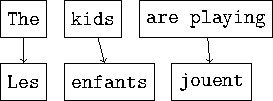
\includegraphics{word_alignment.pdf}
\hspace{0.5cm}
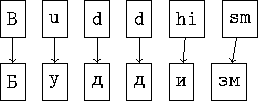
\includegraphics{letter_alignment.pdf}
\end{figure}

\section{Conclusion et perspectives}
\nocite{*}
\bibliographystyle{plain}
\bibliography{report}

\end{document}
